\subsection{Python implementation}
The code is contained in Python classes. The main swapping function is callable as a method class, although the inner loops are split in protected methods, since they are made to work internally. There’s a protected method for each level of depth in the loops of the algorithm described in \ref{section:methods:pipeline}.The information is shared among them via custom objects or the global class attributes.
\\

Aside the main objects, there is a Metadata object which stores all the information for future preprocessing of the data and allows recovery on the same spot the execution ended, either due to an intended halt or an error.
Data for preprocessing is highly important since we require results normalization. This is explained further in the Analysis.

\subsection{Relations Evolution on moving threshold}
\label{suppl:relations}

\begin{figure}[!h]
	\centering
	\begin{subfigure}[b]{0.3\linewidth}
		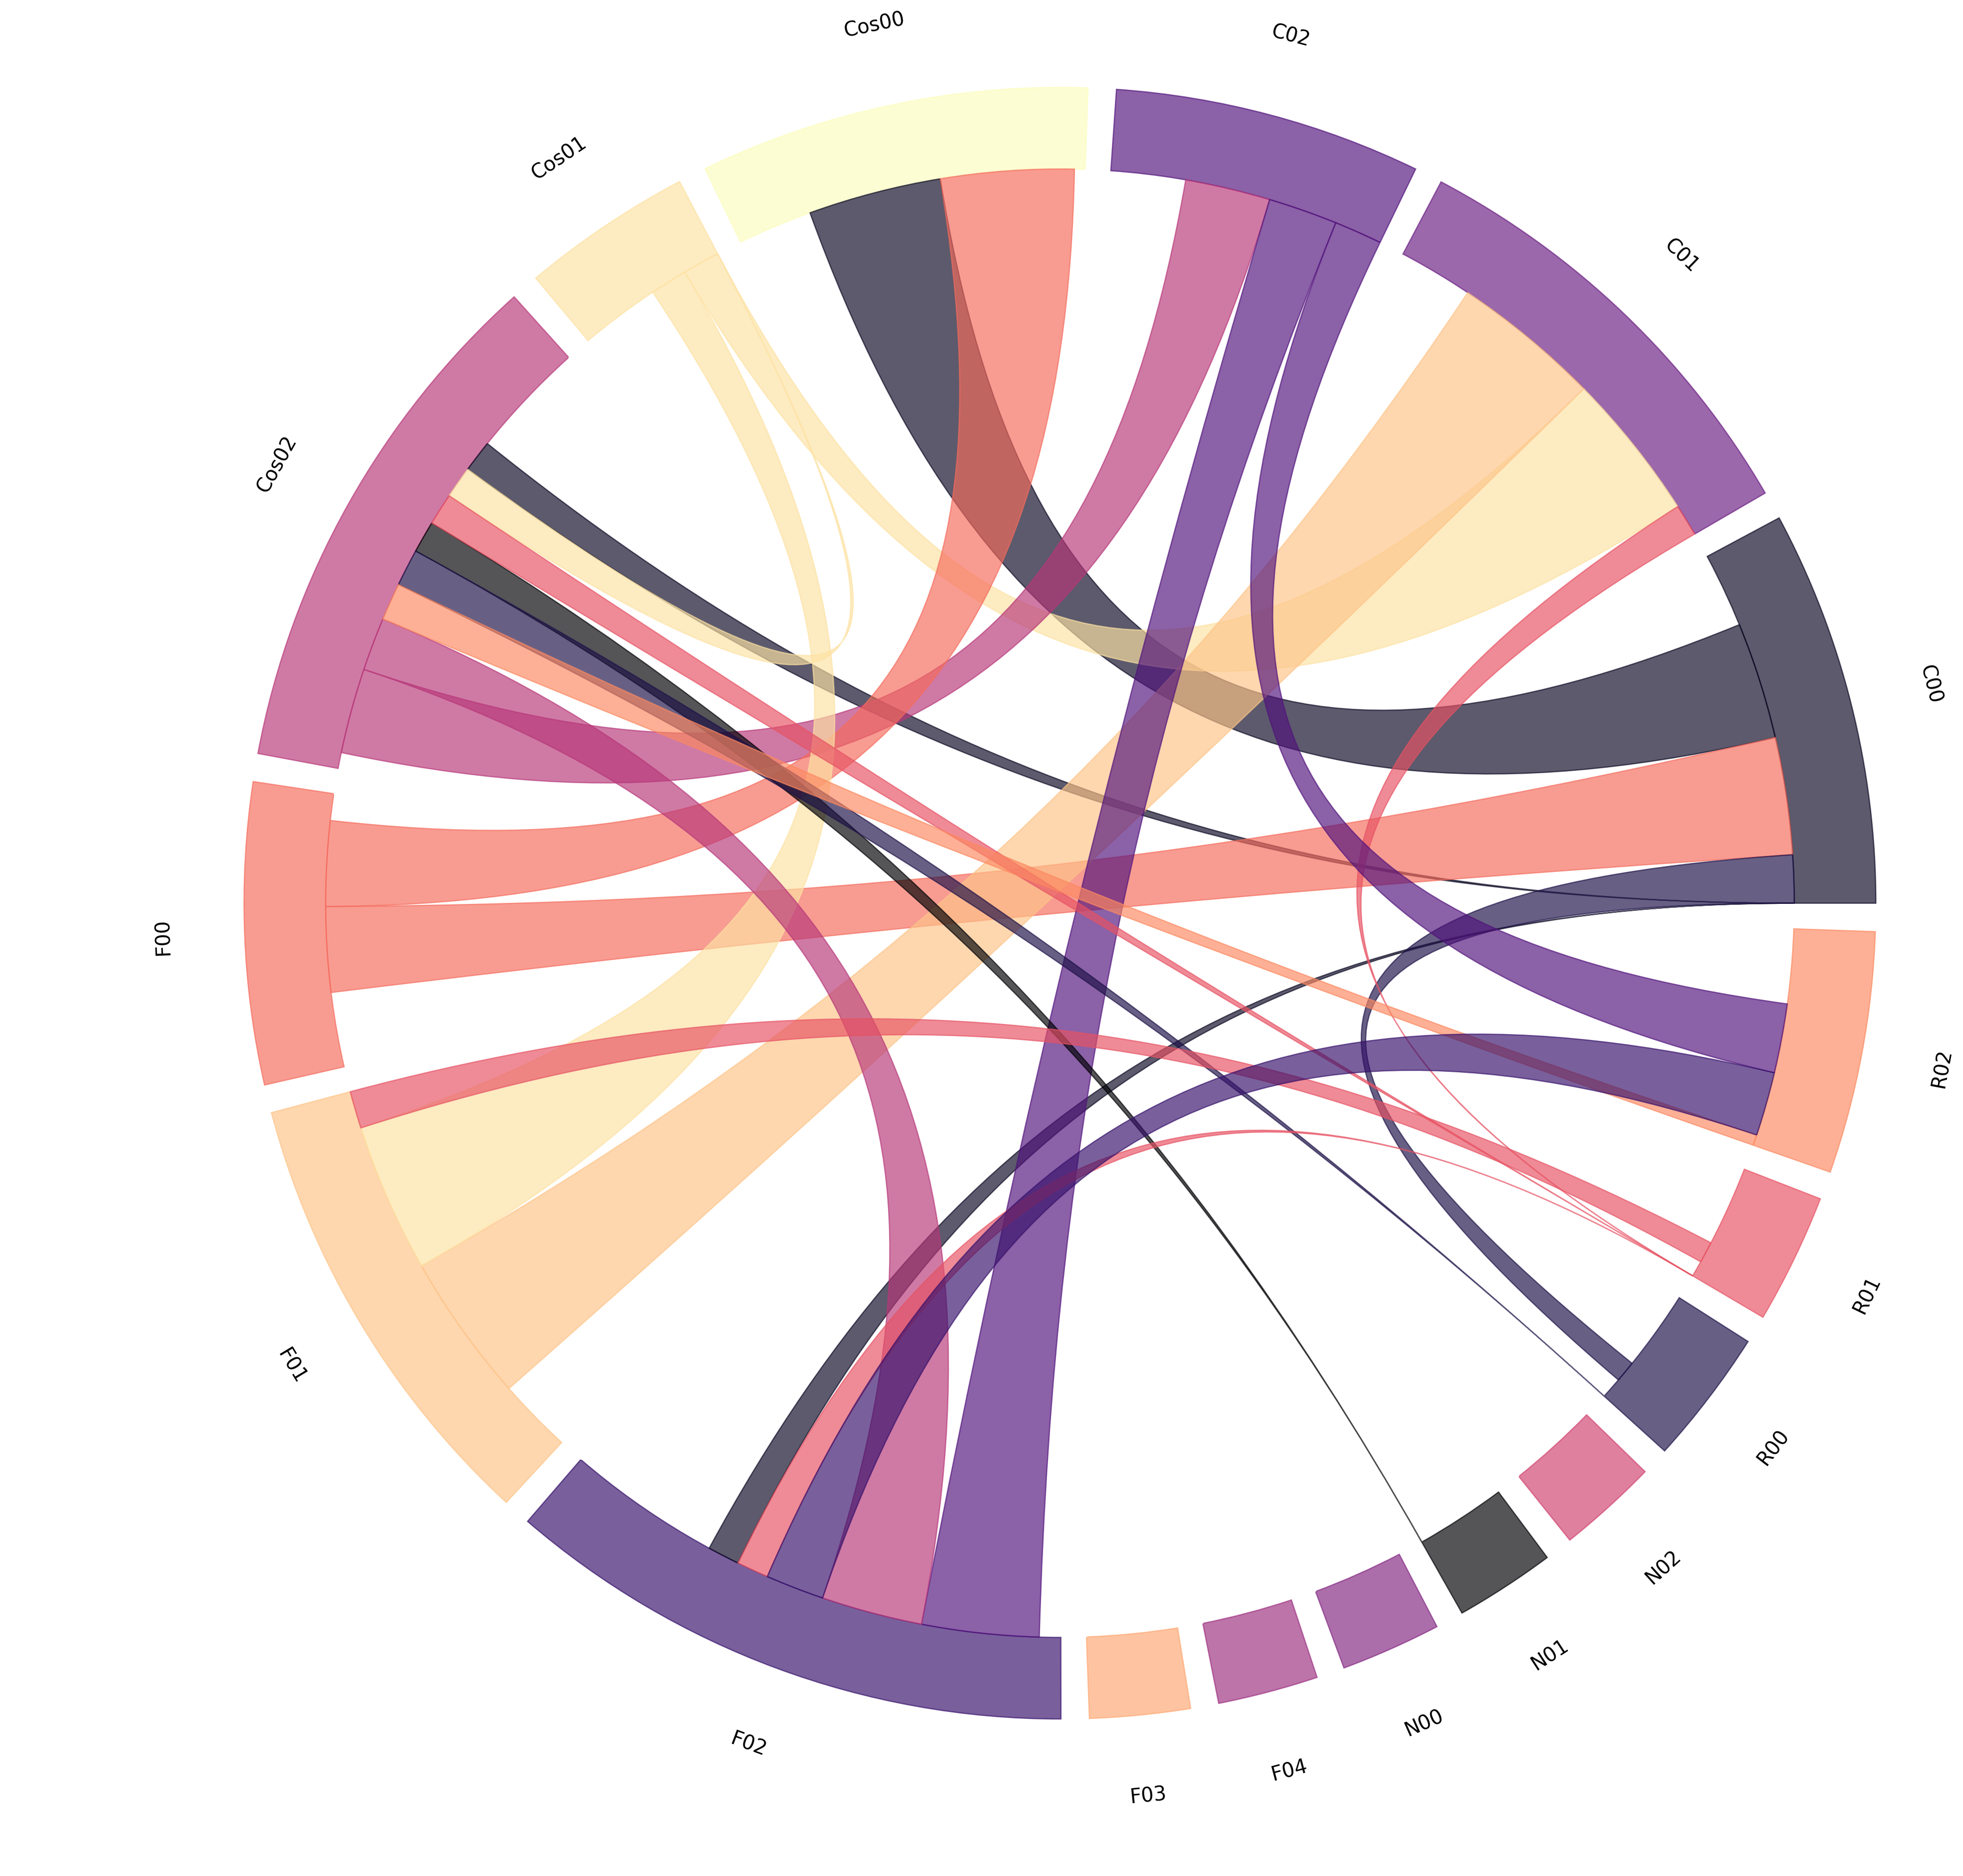
\includegraphics[width=\linewidth]{figures/chords/chord_swap_ensemble1000_RCN5333300_095.png}
		\caption{threshold = 0.95}
	\end{subfigure}
	\hfill
	\begin{subfigure}[b]{0.3\linewidth}
		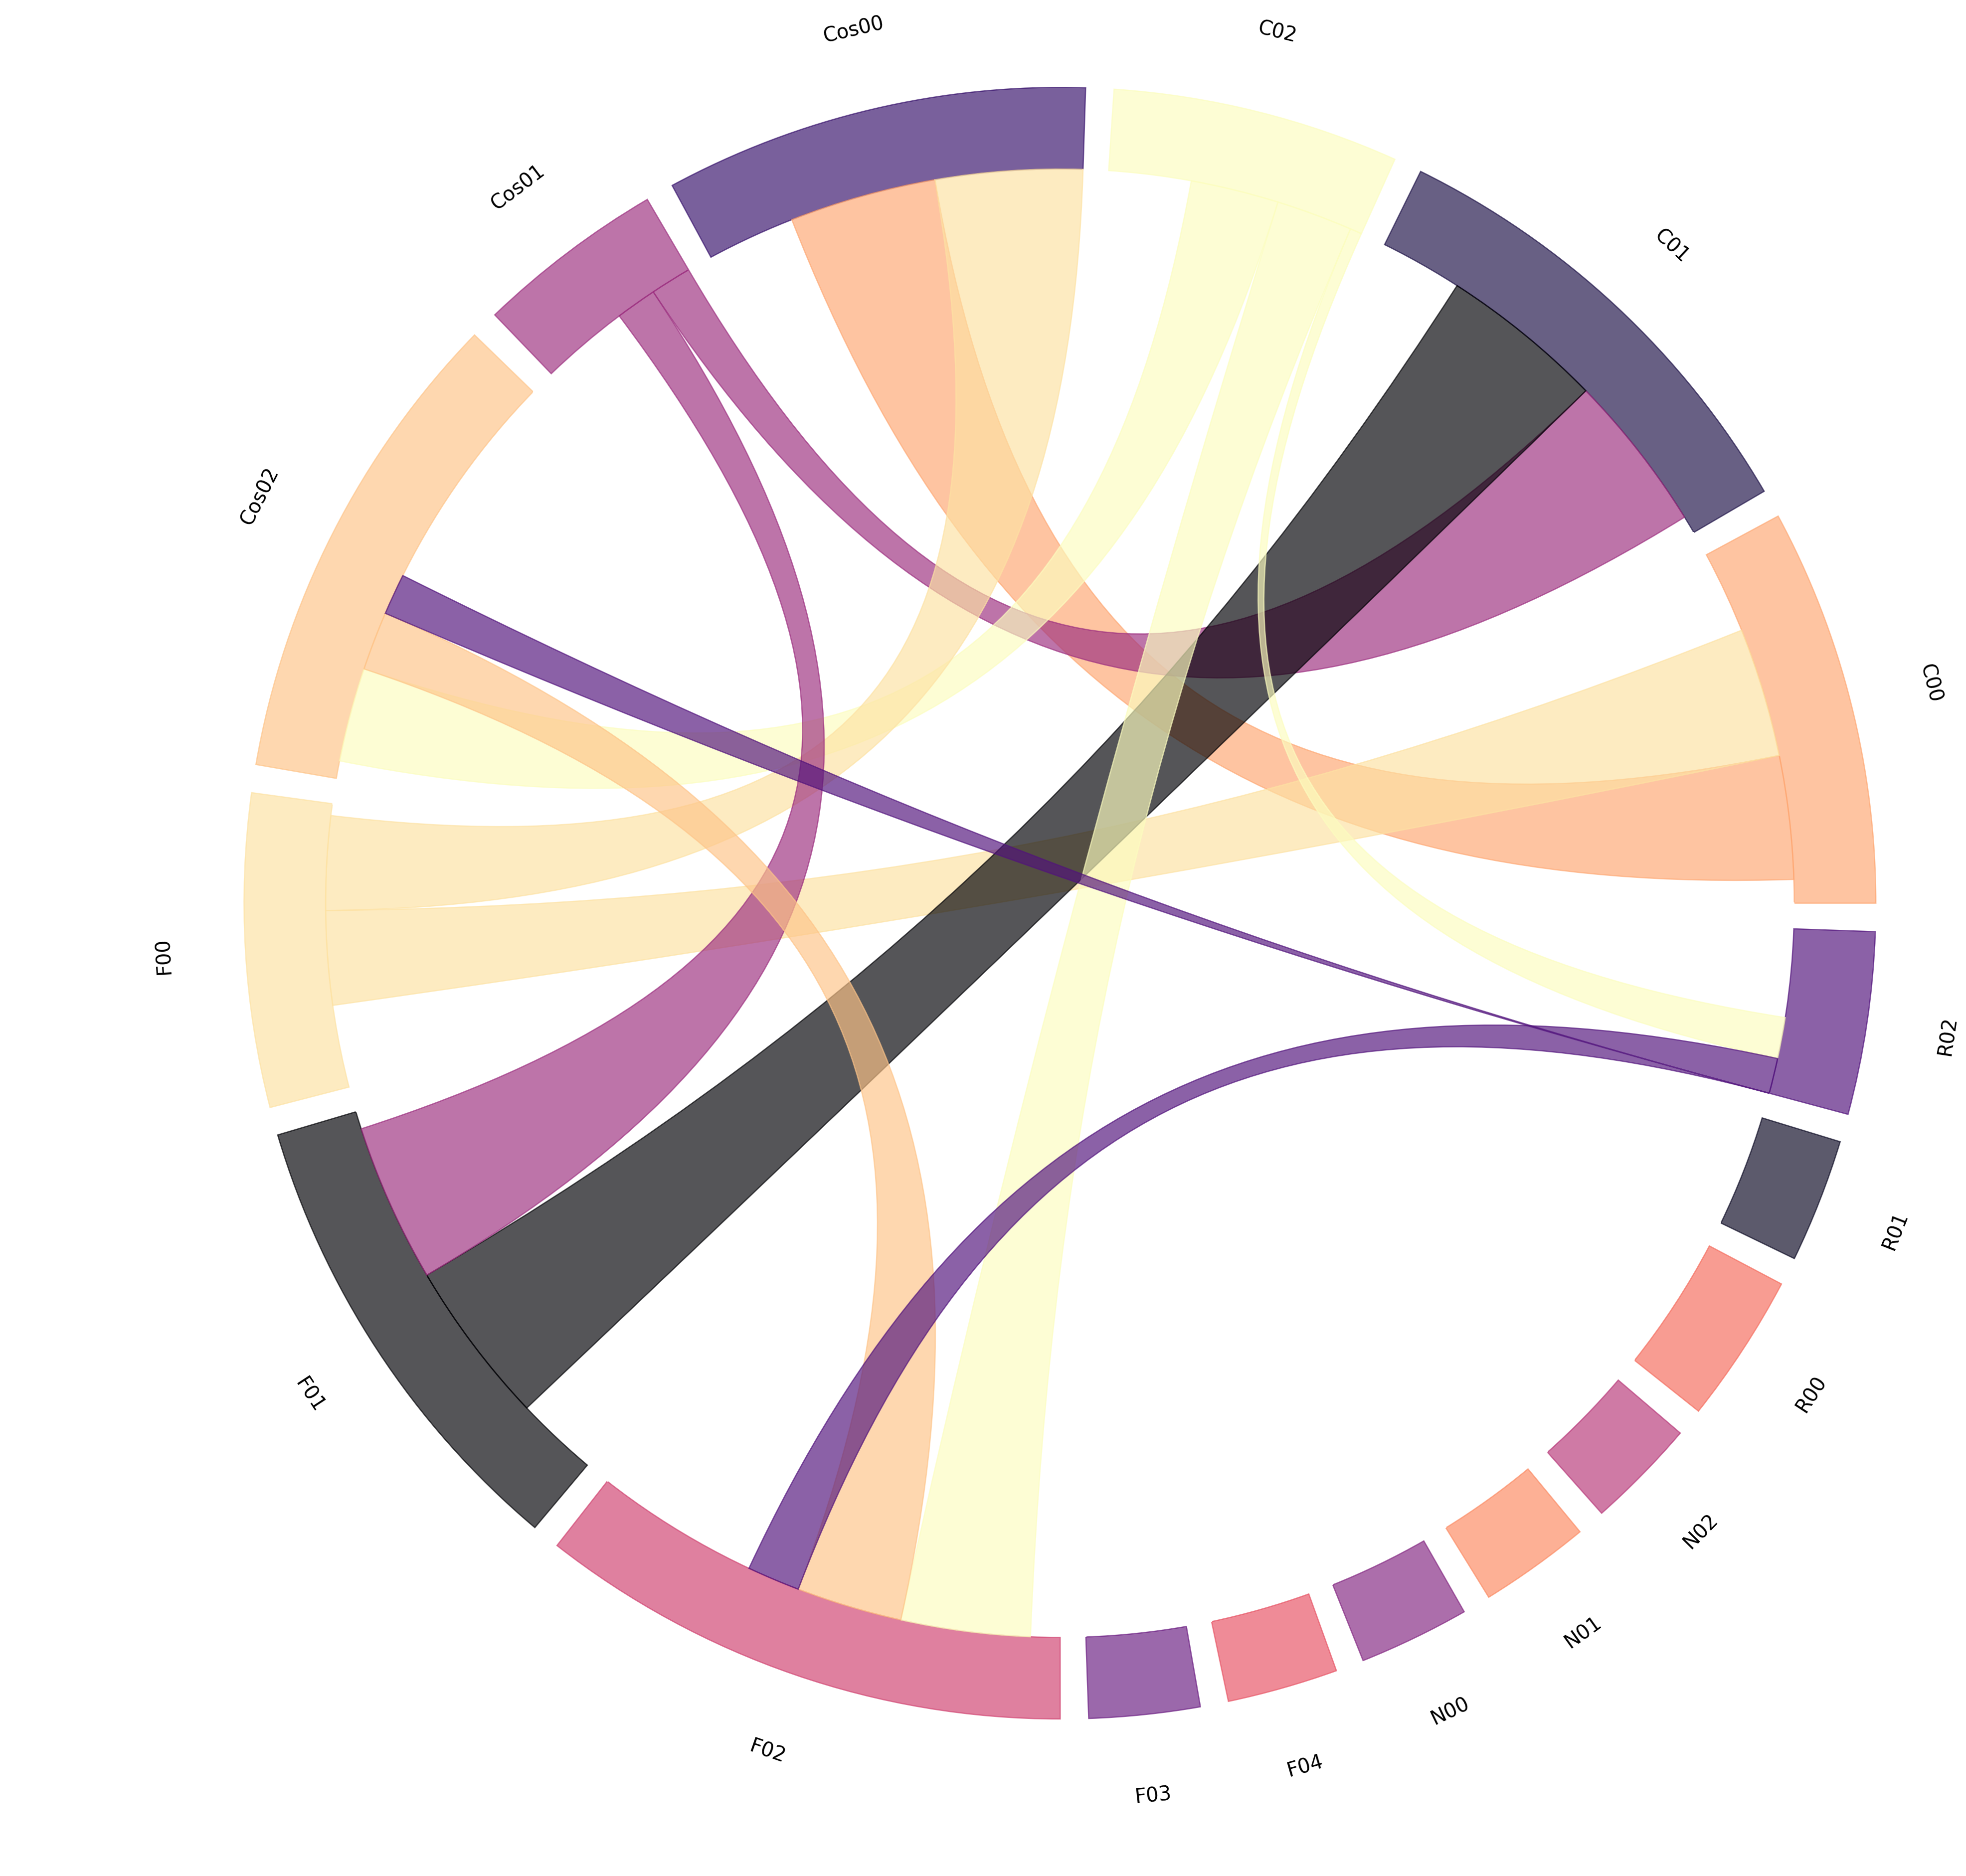
\includegraphics[width=\linewidth]{figures/chords/chord_swap_ensemble1000_RCN5333300_096.png}
		\caption{threshold = 0.96}
	\end{subfigure}
	\hfill
	\begin{subfigure}[b]{0.3\linewidth}
		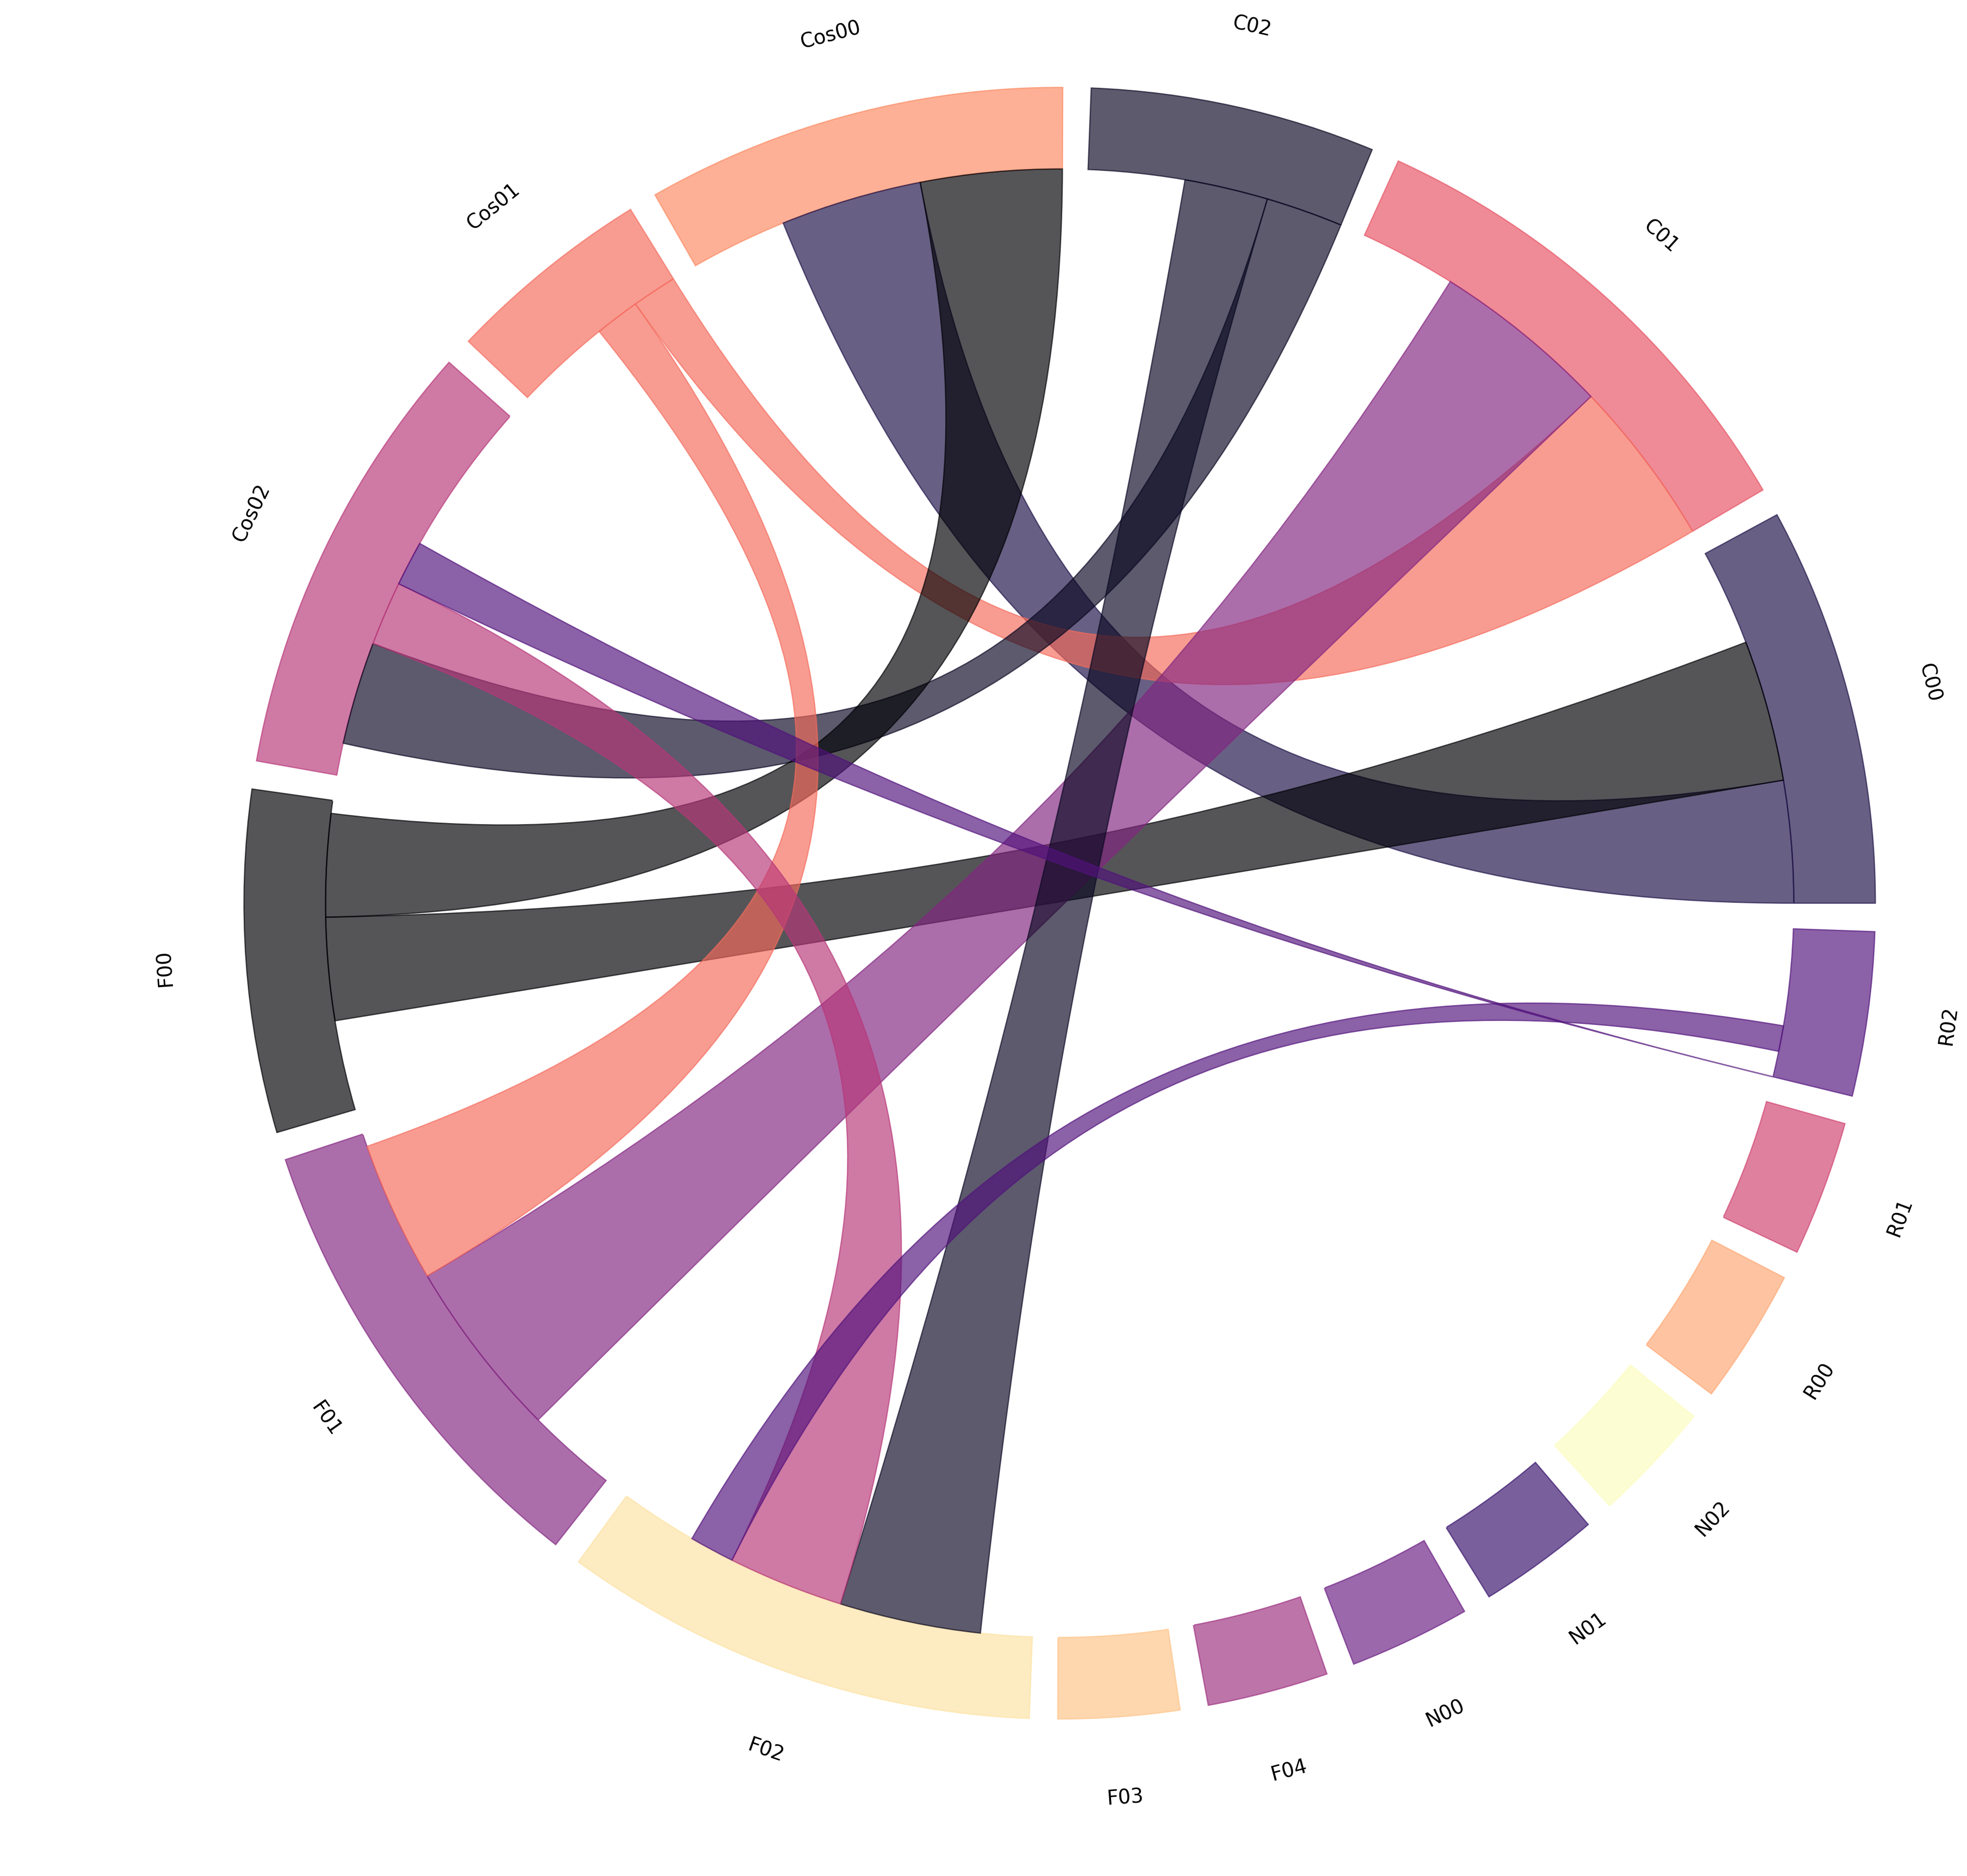
\includegraphics[width=\linewidth]{figures/chords/chord_swap_ensemble1000_RCN5333300_097.png}
		\caption{threshold = 0.97}
	\end{subfigure}
	
	\begin{subfigure}[b]{0.3\linewidth}
		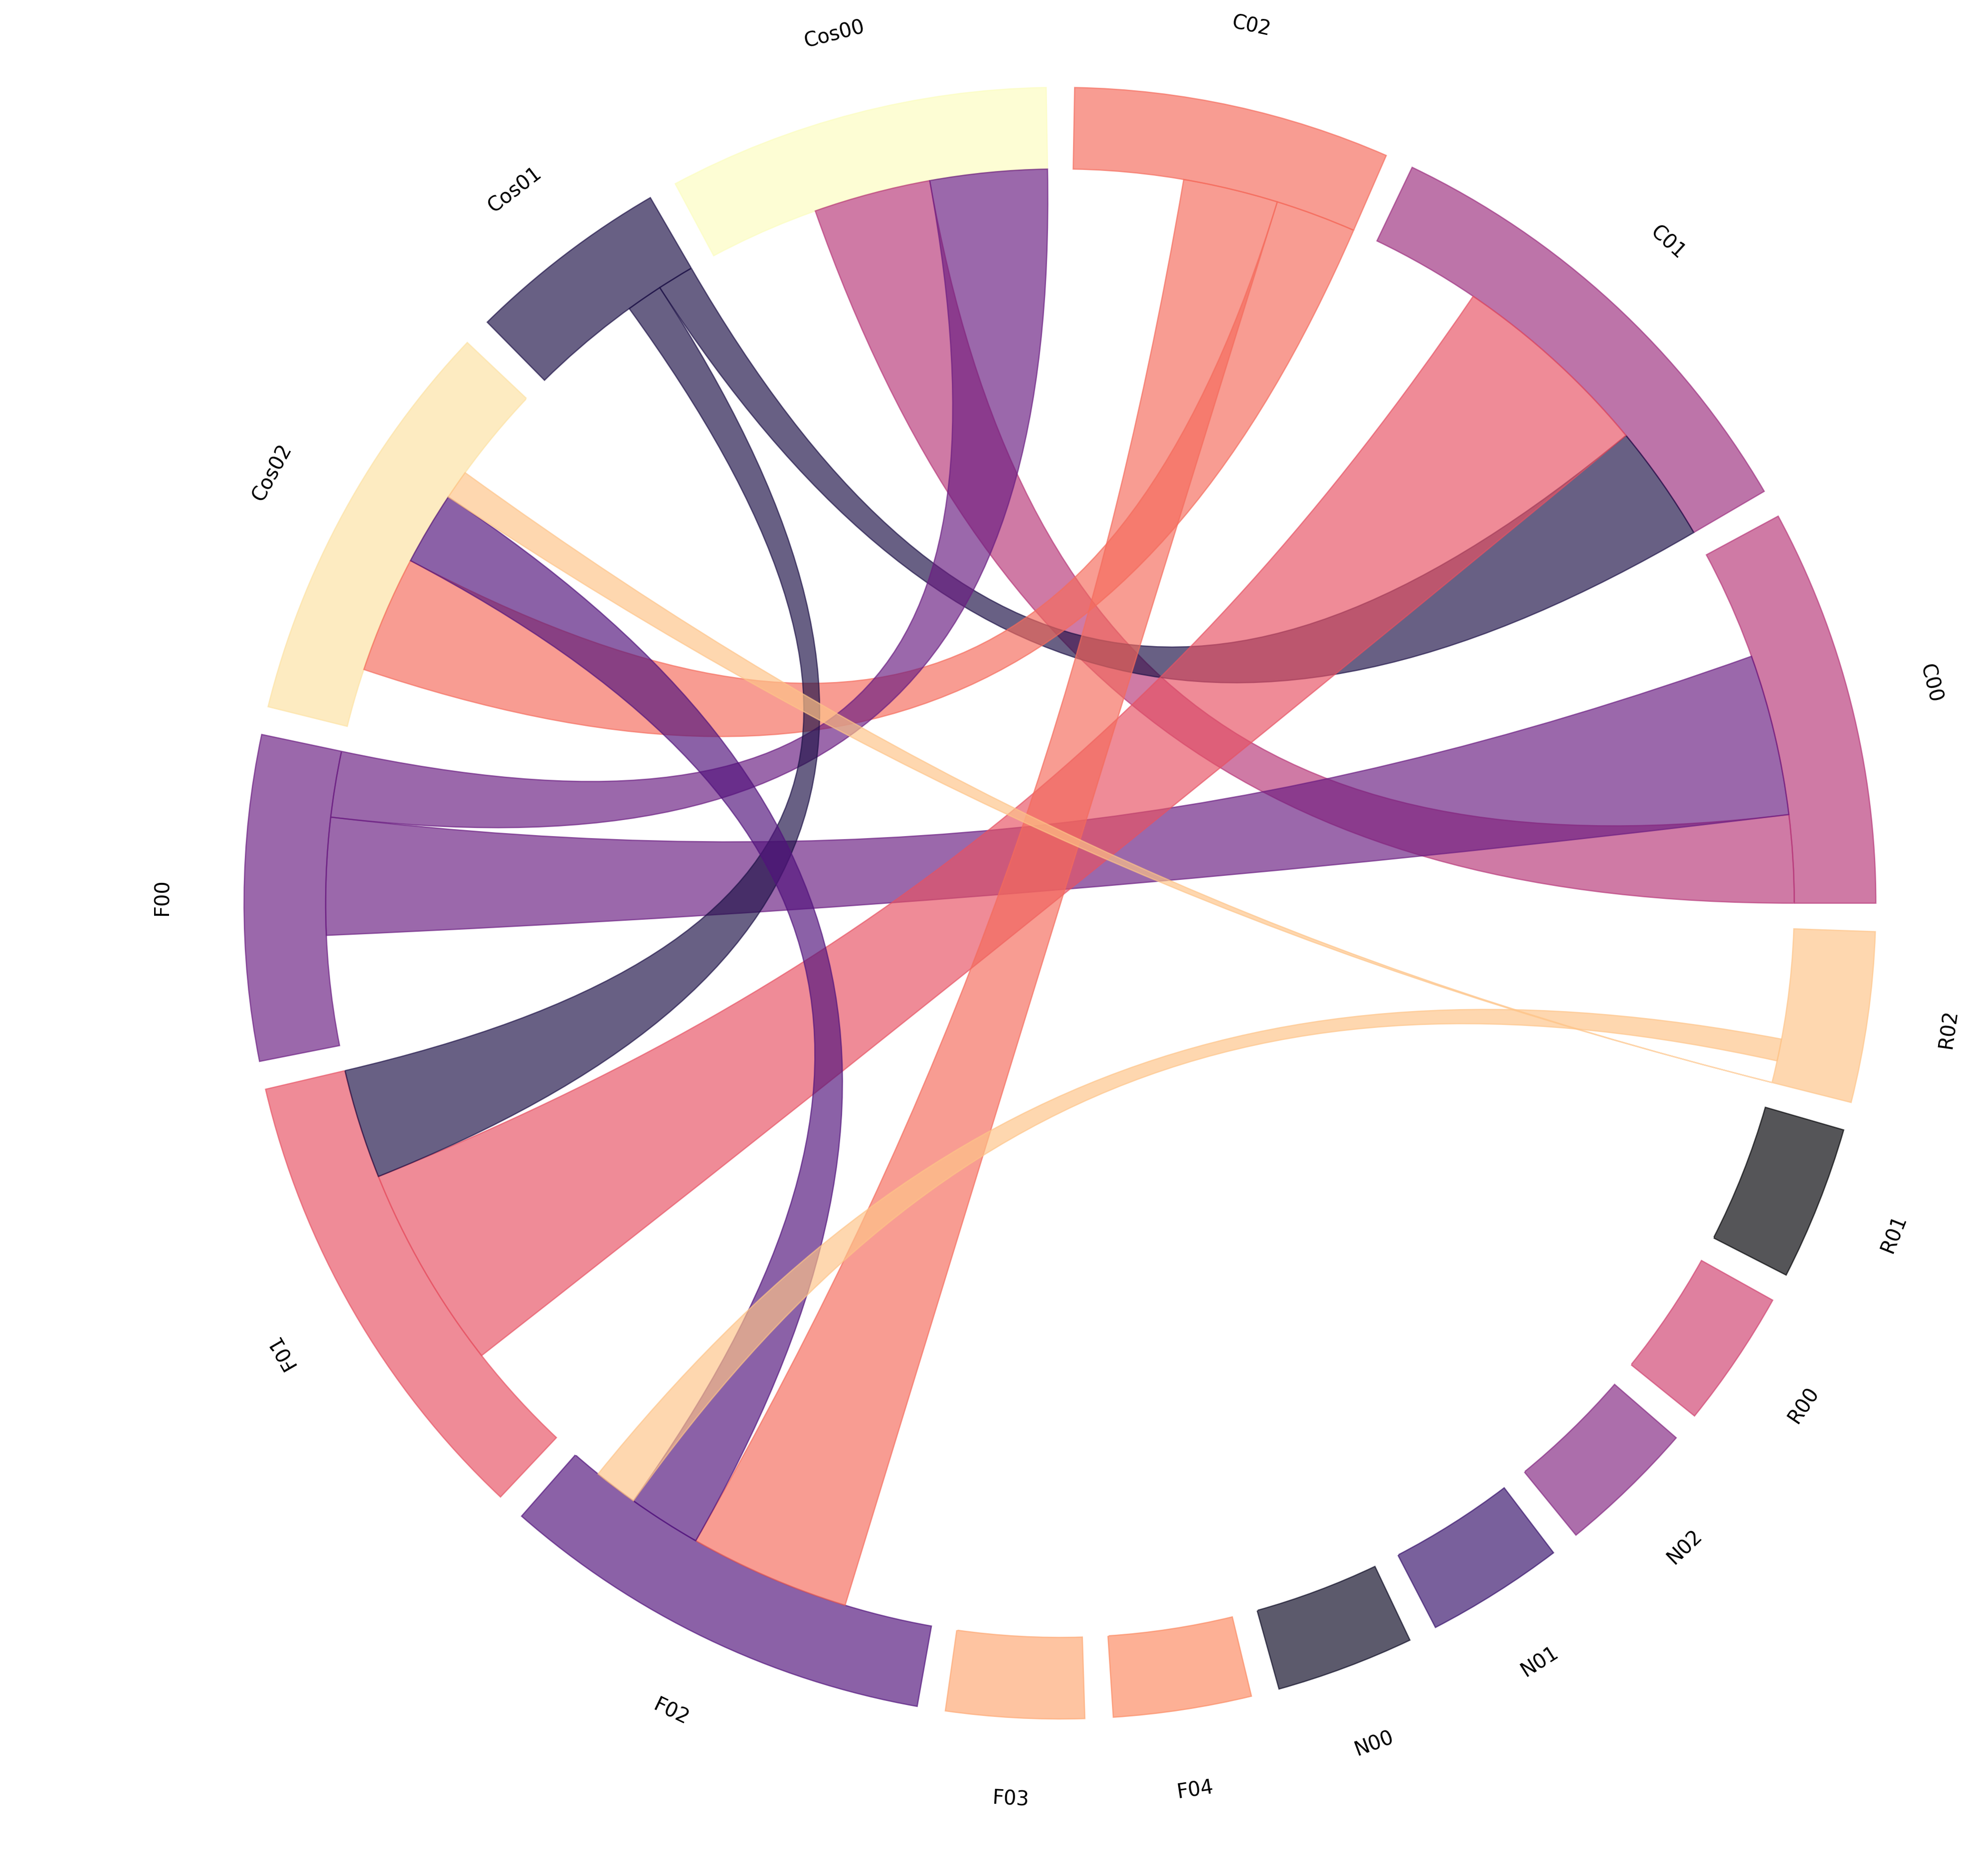
\includegraphics[width=\linewidth]{figures/chords/chord_swap_ensemble1000_RCN5333300_098.png}
		\caption{threshold = 0.98}
	\end{subfigure}
	\hfill
	\begin{subfigure}[b]{0.3\linewidth}
		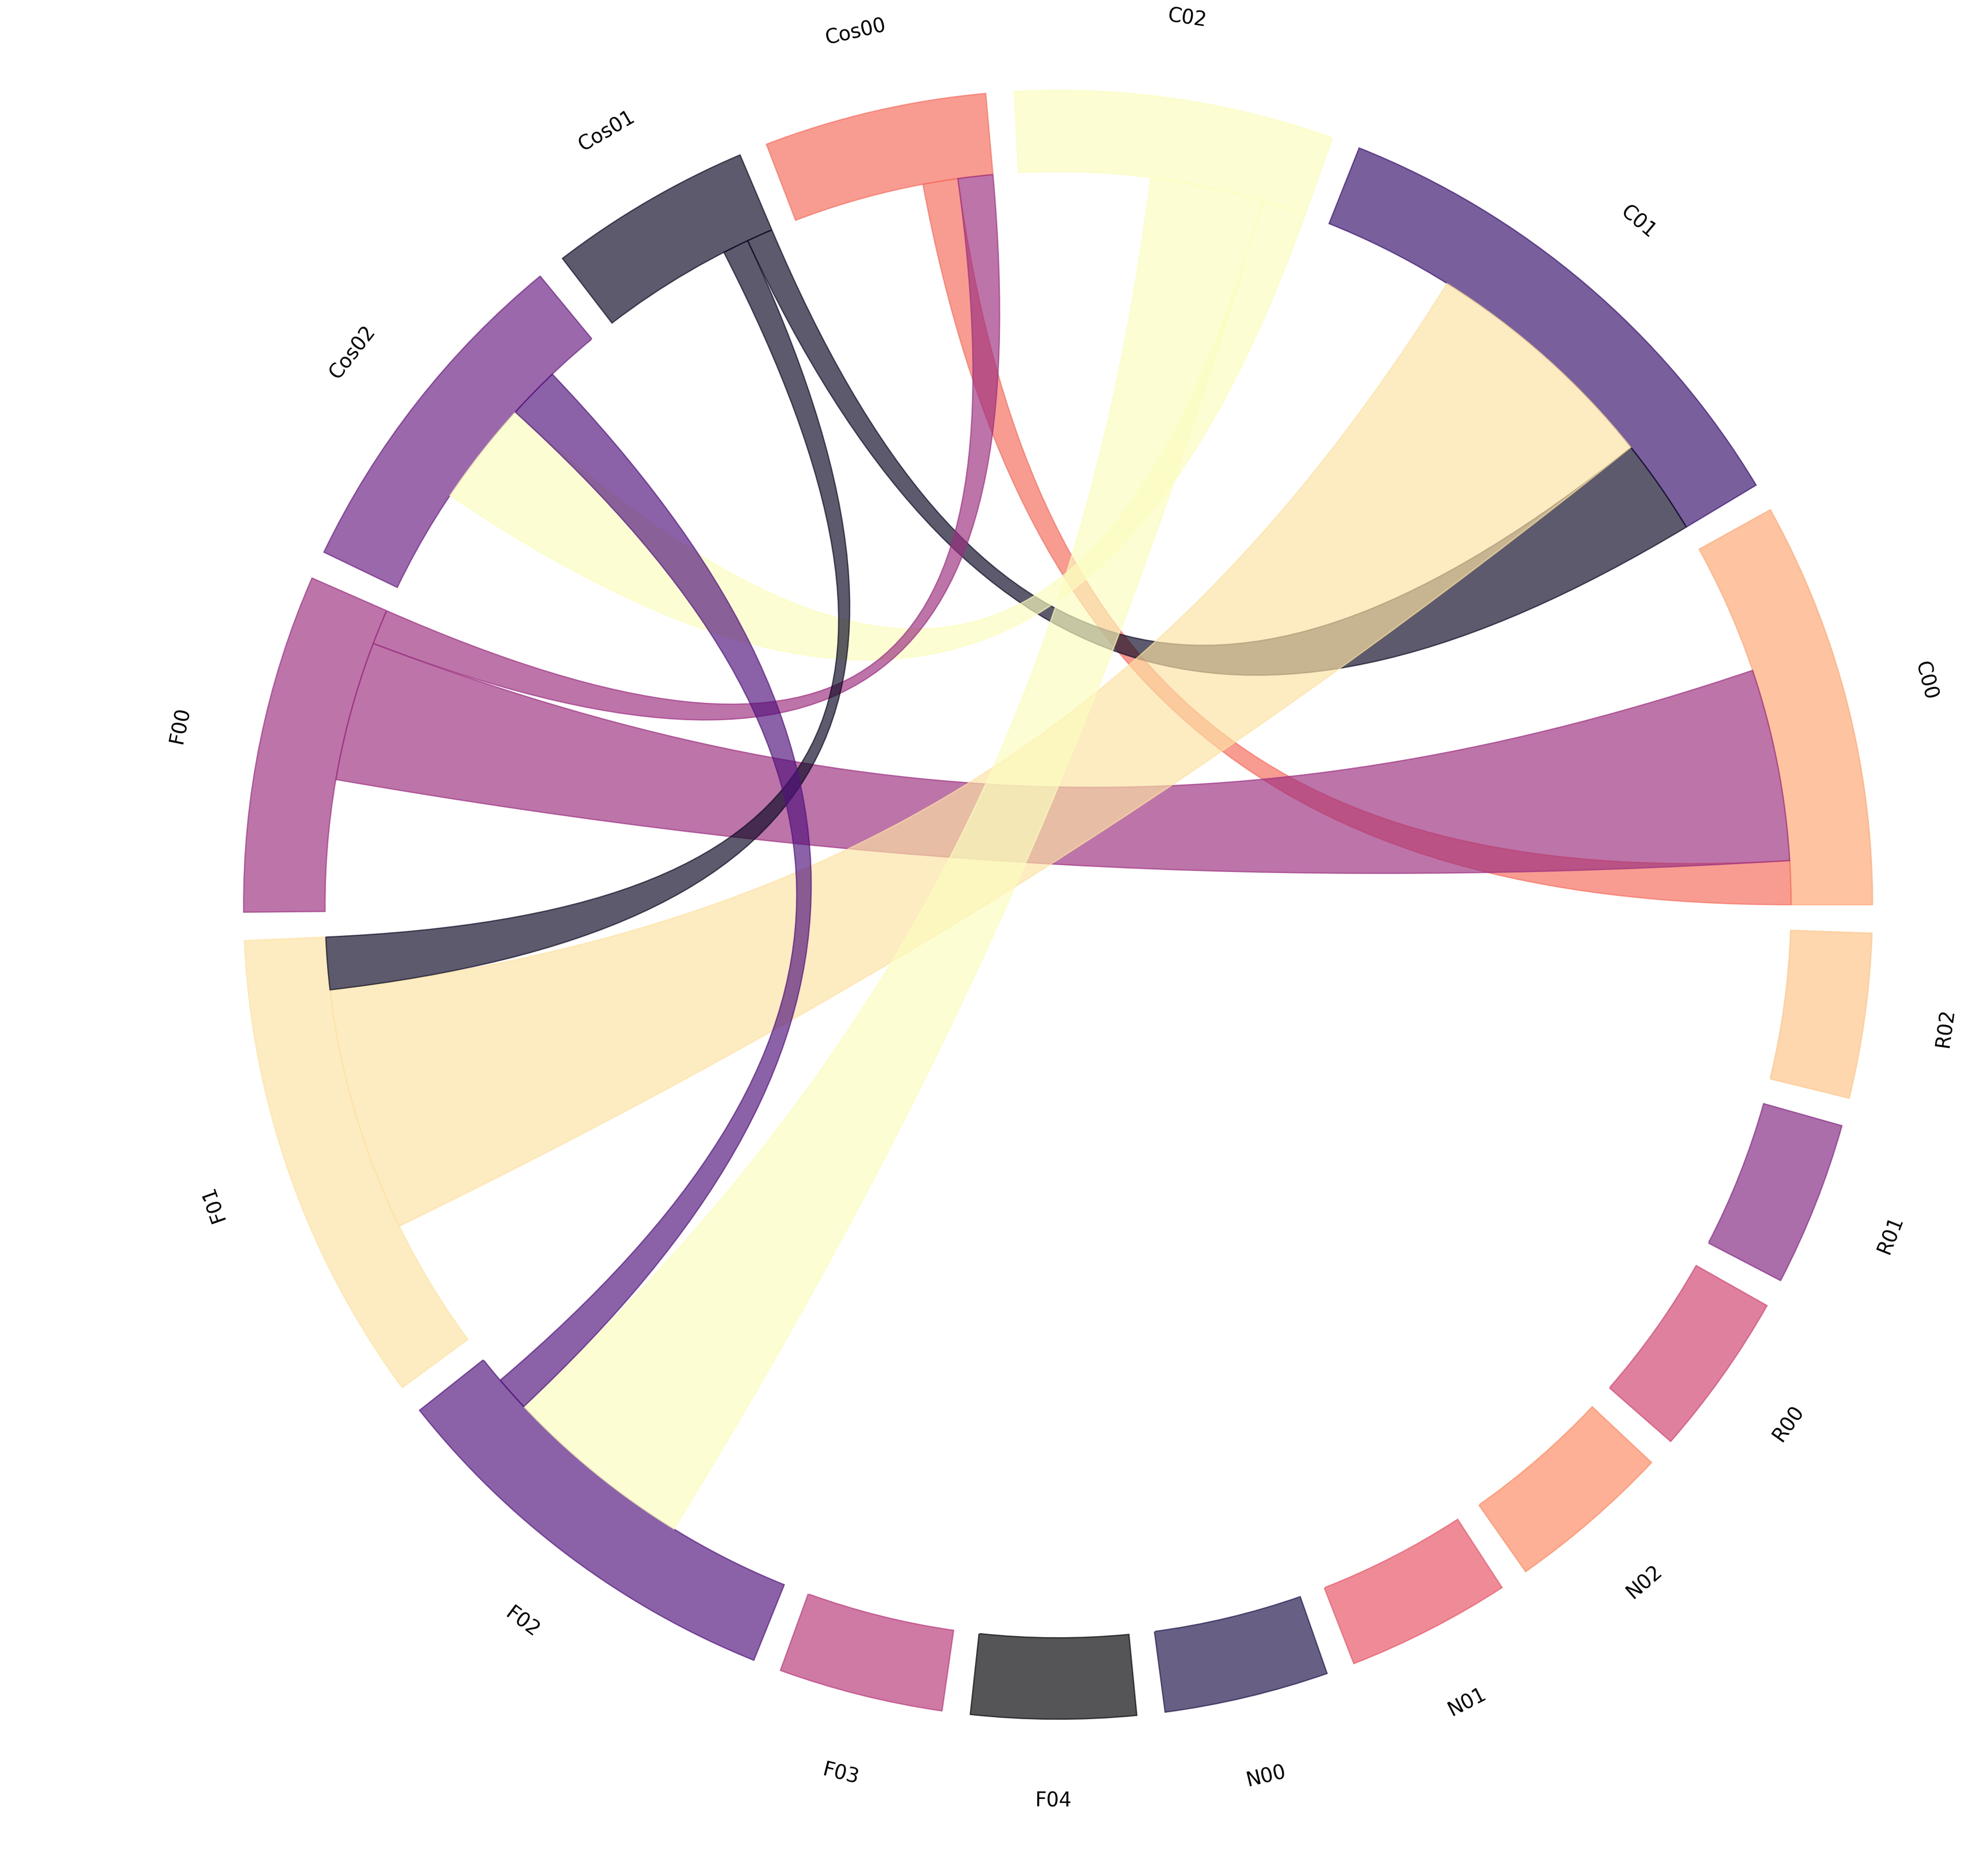
\includegraphics[width=\linewidth]{figures/chords/chord_swap_ensemble1000_RCN5333300_099.png}
		\caption{threshold = 0.99}
	\end{subfigure}
	\hfill
	\begin{subfigure}[b]{0.3\linewidth}
		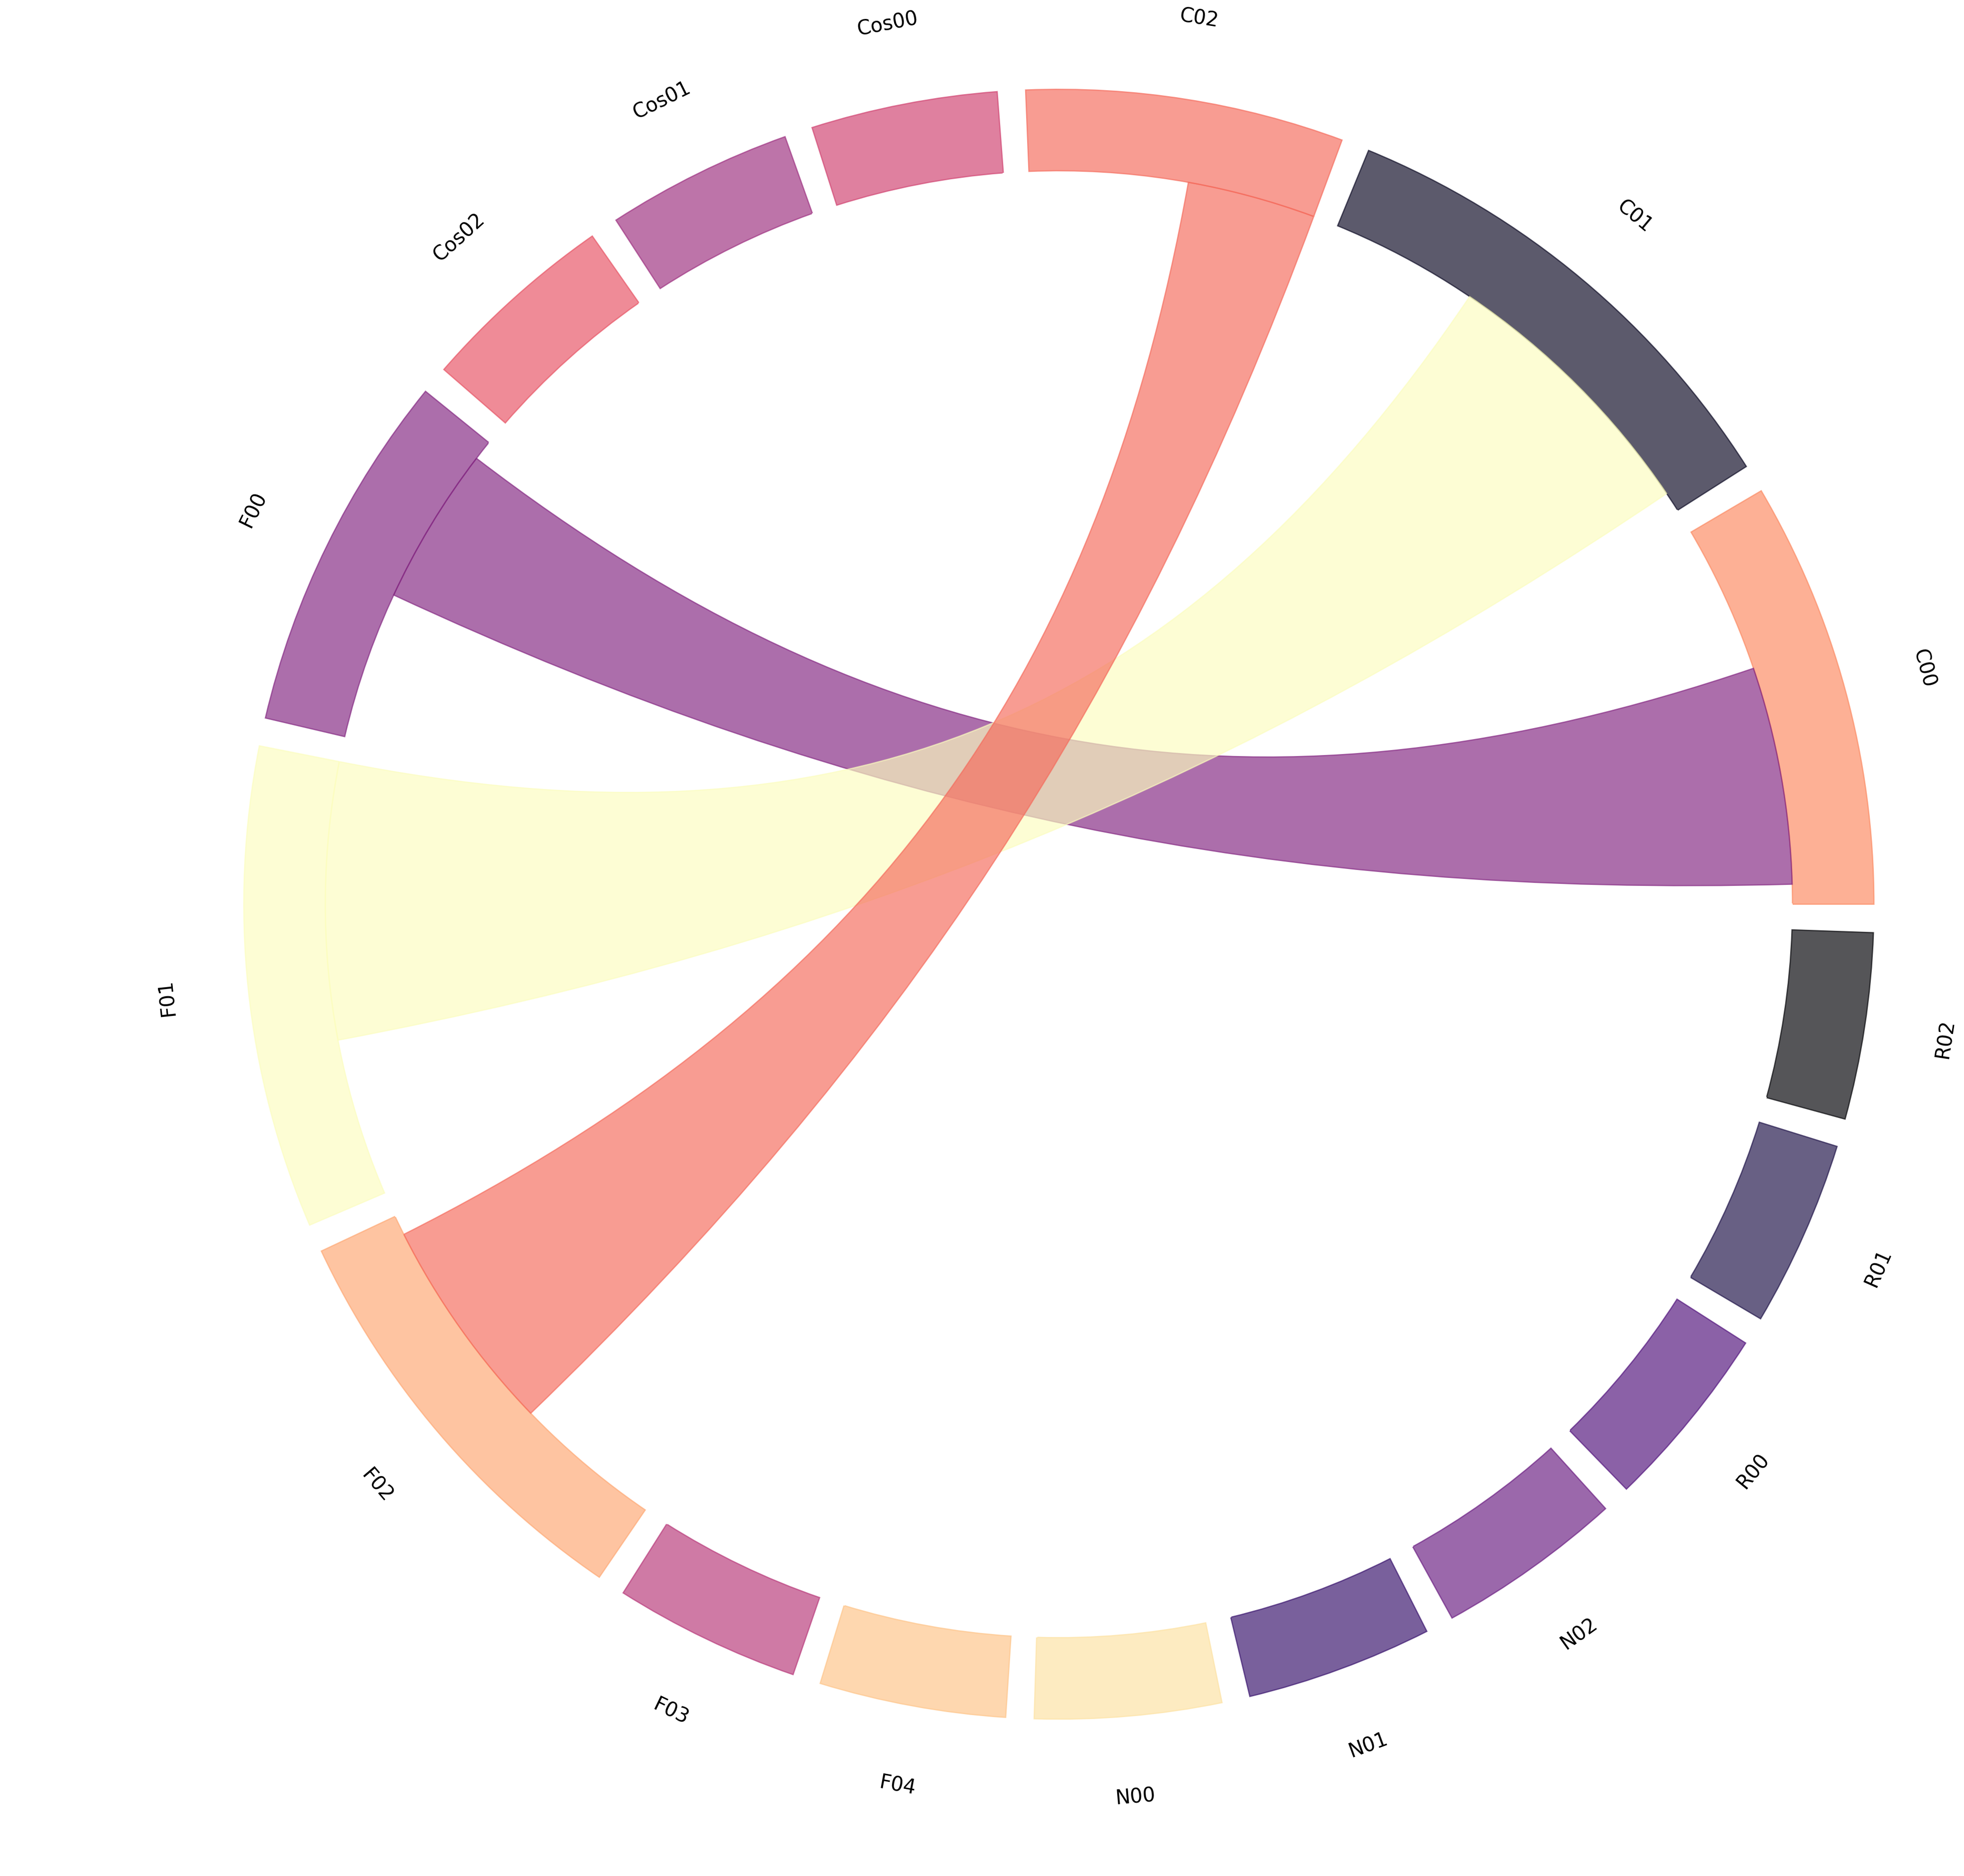
\includegraphics[width=\linewidth]{figures/chords/chord_swap_ensemble1000_RCN53333001.png}
		\caption{threshold = 1}
	\end{subfigure}
	
	\label{fig:tosaqui1}
	\caption{Available relations when increasing the \emph{relation score} threshold.}
\end{figure}